%!TEX root = ../../main.tex
\chapter{Test and Verification}
As already mentioned in previous chapters, the whole EDRICO CPU is designed and implemented in many units. Since the approach using the V-model consists of working in bottom-up order for the implementation, test and verification processes, the first thing to implement and also test are the units of EDRICO. In the following chapters, the bottom-up way of the right side of the V-model (figure \ref{fig:vmod}) is described in detail.
\section{Unit Verification}
The first step in Test and Verification is the Unit Verification. In this step, the lowest units of the project are tested to prevent possible bugs from occurring in later stages of the verification. It is crucial to test every unit of the project because in a later stage of verification it is very complicated and time intensive to localize the bug and fix it in a top-down way. The main goal is to identify and fix bugs as early as possible. In this section, the unit verification process for the CU decoding unit is described in detail.\\
The task of the decoding unit is to parse the 32-bit instruction string, extract information and set the control signals respectively.\\
Unit verification starts by inserting source files of the implementation into a Xilinx Vivado\textcopyright  project. To test a unit, it is required to implement a so called testbench. This testbench will serve as a test environment for the \ac{UUT}. Testbenches are used for simulation purpose only (not for synthesis). Therefore, several VHDL constructs like \textit{assert}, \textit{report}, or \textit{loop} can be used. During the testbench simulation, the UUT is stimulated with different input data. In this case, the decoder receives a different 32-bit instruction string. The following code shows how the stimulation process is implemented:
\begin{lstlisting}[style=vhdl, caption=CU testbench stimulation process]
stim: process
begin
	-- parse through different instruction strings
	--OPIMM
	ir <= "00000000001000100000000010010011"; --ADDI
	wait for 100ns;
	ir <= "00000000001000100010000010010011"; --SLTI
	wait for 100ns;
	ir <= "00000000001000100011000010010011"; --SLTIU
	wait for 100ns;
	ir <= "00000000001000100100000010010011"; --XORI
	...
\end{lstlisting}
To verify the functionality of the decoder unit, Vivado generates a timing diagram where it is possible to inspect all input and output signals of the UUT. The following figure \ref{fig:opimm} shows the timing diagram for the CU decoder testbench.
\begin{figure}[H]
	\centering
	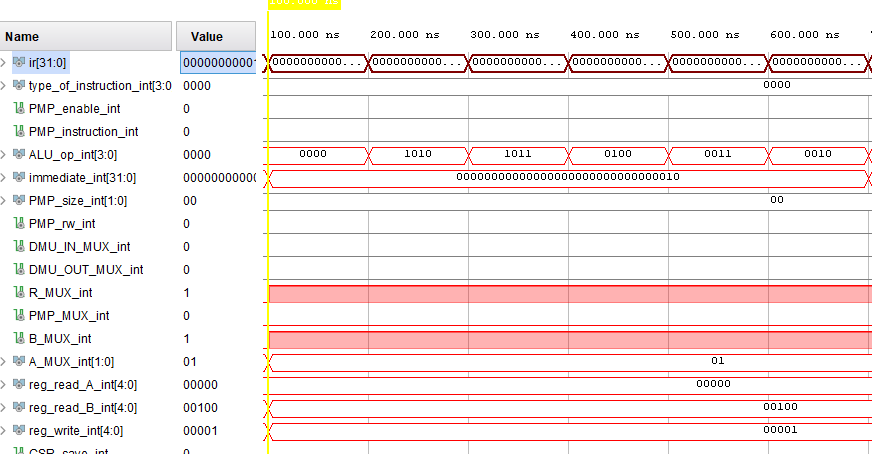
\includegraphics[width=\textwidth]{CUtbOPIMM}
	\caption{Vivado timing diagram for OPIMM instructions}
	\label{fig:opimm}
\end{figure}
For the OPIMM instruction cluster, the relevant output signals are highlighted in red. The top row shows how the instruction string is changing every 100 ns. As a result of that, the \textit{ALU\_op} signal changes, as the instruction changes. The first instruction is a \textit{ADDI} instruction which should lead to a 4-bit output signal of \textbf{0000}. After that a \textit{SLTI} instruction is inserted which should lead to a \textbf{1010} output (as shown in table \ref{aluop}). These outputs are correctly set as the timing diagram shows. The same validation technique is executed for all the other relevant signals. After establishing a correct signal for every output and every instruction, the unit can be declared as verified.\\
Figure \ref{fig:cutiming} shows the full timing diagram for the full testbench duration. It is visible that for example the memory signals are only active for memory operations.
\begin{figure}[H]
	\centering
	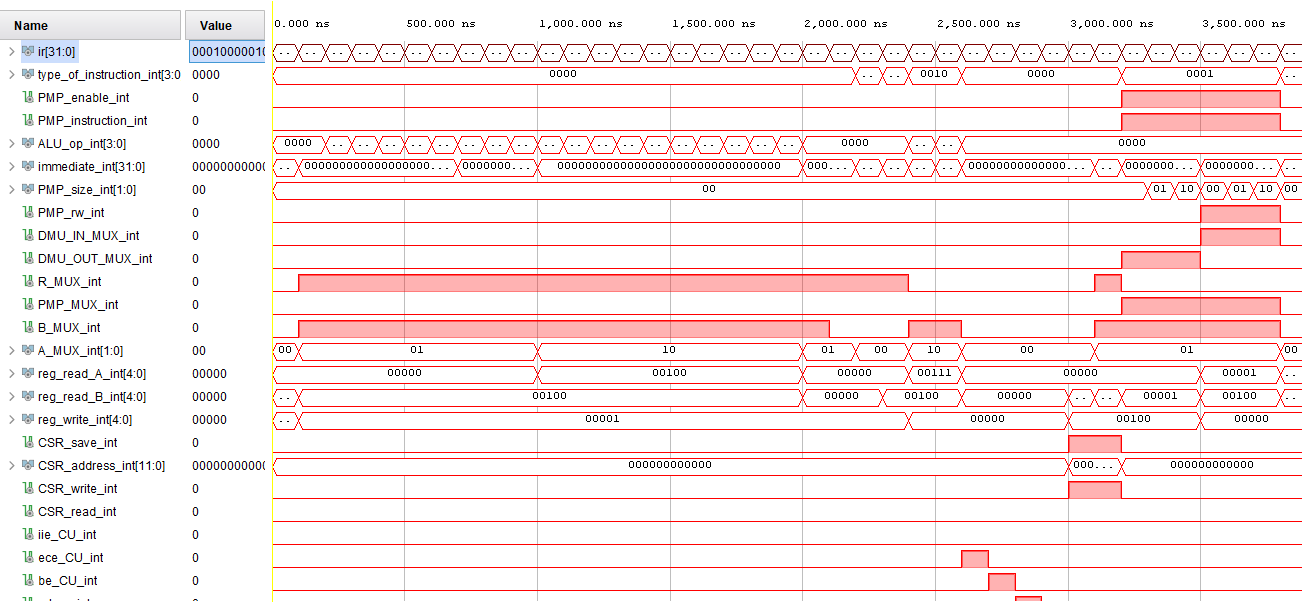
\includegraphics[width=\textwidth]{CUtiming}
	\caption{Vivado timing diagram for full CU decoder testbench}
	\label{fig:cutiming}
\end{figure}

Another unit that had to be verified outside of the control unit is the ALU. Since the complexity of the ALU is not as high as of the control unit, the testbench and also the timing diagram are very simple. The stimulation process of the ALU testbench is shown in the code below:
\begin{lstlisting}[style=vhdl, caption=ALU testbench stimulation process]
stim: process
begin
	-- set input signal
	in_a <= "00000000000000000000000000000010";
	in_b <= "00000000000000000000000001000000";

	-- set op signal
	alu_op <= "0000"; --ADD
	wait for 100ns;
	alu_op <= "0001"; --SUB
	wait for 100ns;
	alu_op <= "0010"; --AND
	wait for 100ns;
	alu_op <= "0011"; --OR
	wait for 100ns;
	alu_op <= "0100"; --XOR
	wait for 100ns;
	alu_op <= "0101"; --EQUAL
	wait for 100ns;
	alu_op <= "0110"; --NEQUAL
	wait for 100ns;
	alu_op <= "0111"; --shift_left
	wait for 100ns; 
	alu_op <= "1000"; --shift_right
	wait for 100ns;
	alu_op <= "1001"; --shift_right (arithmetic)
	...
\end{lstlisting}
This code shows the first few operations that the ALU performs. First of all a pre defined input is fed to the ALU consisting of \textit{in\_a = 0x00000002} and \textit{in\_b = 0x00000040}. With these inputs, the different ALU operations are called using the \textit{alu\_op} signal. The following table \ref{table:alutb} will give an overview over what the expected results are:
\begin{table}[H]
	\setlength\arrayrulewidth{2pt}
	\centering
	\begin{tabular}{|c|c|c|}
		\hline
		\rowcolor{light-gray}
		\textbf{ALU\_OP} & \textbf{ALU\_result} & \textbf{branch\_re} \\
		\hline
		0000 (ADD) & 0x00000042 & 0 \\
		\hline
		0001 (SUB) & 0x0000003e & 0 \\
		\hline
		0010 (AND) & 0x00000000 & 0\\
		\hline
		0011 (OR) & 0x00000042 & 0\\
		\hline
		0100 (XOR) & 0x00000042 & 0\\
		\hline
		0101 (EQUAL)& 0x00000000 & 0\\
		\hline
		0110 (NEQUAL)& 0x00000000 & 1\\
		\hline
		0111 (shift\_left) & 0x00000100 & 0\\
		\hline
		1000 (shift\_right)& 0x00000010 & 0 \\
		\hline
		1001 (shift\_right (arith.))& 0x00000010 & 0\\
		\hline
	\end{tabular}
	\label{table:alutb}
	\caption{ALU testbench correct outputs}
\end{table}
The branch\_re output is only relevant for operations that can be called by branch instructions. In this case, the \textit{EQUAL} and \textit{NEQUAL} operations have to deliver a branch response. Since the two inputs are not the same, the \textit{EQUAL} operation shall return 0 while the \textit{NEQUAL} operation shall return 1. The other operations are basic mathematical and arithmetical operations and the output is calculated by just performing the respective operations on the two inputs. After simulating the testbench in Vivado the resulting timing diagram (figure \ref{fig:alutb}) shows that everything works as desired. 
\begin{figure}[H]
	\centering
	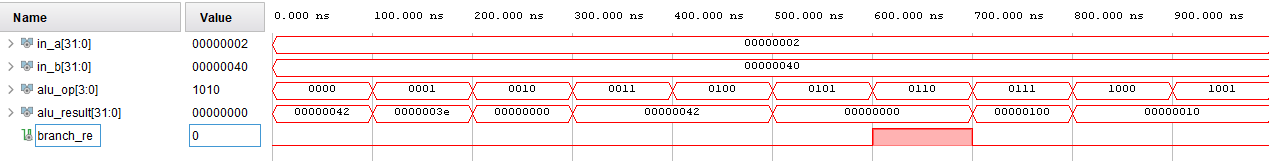
\includegraphics[width=\textwidth]{ALUtb}
	\caption{Vivado timing diagram for ALU testbench}
	\label{fig:alutb}
\end{figure}
With the same approach, every other unit is verified and occuring bugs are fixed until simulation and desired output are equal.
\section{Integration Verification}
During this stage of Test and Verification, all of the units have already been tested and verified. In this step, it is verified, that the units created and tested independently can coexist and communicate among themselves. In this project, the Integration Verification consists of creating so called \textit{top-files} which conclude all the corresponding units to a sub system. This section describes how the Control Unit of the EDRICO CPU went through this stage.\\
Since the CU consists of the units \textit{CU\_decoder, CU\_execute\_enable, CU\_FSM and CU\_PC}, the top file gets very big since it combines and connects all the mentioned units. As shown in figure \ref{fig:cuarchitecture} there are a lot of control signals going out of the control unit and some signals going in. These inputs and outputs are the only signals visible from the 'outside' and therefore are the only signals to be monitored during testing. Since all units are already verified, the internal communication and processing should be working correctly. The creation of the testbench for this integration is much more complex than the testing for the single units. Since the timing of the state machine is working autonomously, the input signal manipulation has to be adapted respectively. Due to this high complexity, a package file was created to outsource input signal manipulation and also output signal monitoring.\\
In this package file, there are multiple vectors consisting of the different input signals and the desired output signals. An example for these vectors is shown in the code below:
\begin{lstlisting}[style=vhdl, caption=CU top testbench package]
type data_stim is array(natural range <>) of std_logic_vector(31 downto 0);
type result_vec is array(natural range <>) of std_logic_vector(149 downto 0);

constant instruction : data_stim(38 downto 0) :=
	(
	1 => "00000000001000100000000010010011",    --ADDI
	2 => "00000000001000100010000010010011",    --SLTI
	3 => "00000000001000100011000010010011",    --SLTIU
	...
	22 => "00000100000100001001000011101111",   --JAL
	23 => "00000010101000100000000011100111",   --JALR
	24 => "10000010011100100000100011100011",   --BEQ
	29 => "00010000010100000000000001110011",   --WFI
	30 => "00000000010000110001001001110011",   --CSRRW
	...
constant results : result_vec(38 downto 0) :=
	(
	1 => x"00220093" & x"00000008" & '0' & '0' & "00" & '0' & '0' & '0' & '1' & '0' & '1' & "01" & "00000" & "00100" & "00001" & "000000000000" & '0' & '0' & '0' & "0000" & "100" & '0' & '0' & '0' & '0' & x"00000002" & '1',    --ADDI
	...
	10 => x"004200B3" & x"0000002C" & '0' & '0' & "00" & '0' & '0' & '0' & '1' & '0' & '1' & "10" & "00100" & "00100" & "00001" & "000000000000" & '0' & '0' & '0' & "0000" & "100" & '0' & '0' & '0' & '0' & x"00000000" & '1',   --ADD
	...
	 26 => x"00000073" & x"00000000" & '0' & '0' & "00" & '0' & '0' & '0' & '0' & '0' & '0' & "00" & "00000" & "00000" & "00000" & "000000000000" & '0' & '0' & '0' & "0000" & "100" & '0' & '1' & '0' & '0' & x"00000000" & '1',   --ECALL
	 ...
	 35 => x"00120423" & x"00000000" & '1' & '1' & "00" & '1' & '1' & '0' & '0' & '1' & '1' & "01" & "00001" & "00100" & "00000" & "000000000000" & '0' & '0' & '0' & "0000" & "001" & '0' & '0' & '0' & '0' & x"00000008" & '1',   --SB
	 ...
\end{lstlisting}
The \textit{instruction} vector of type \textit{data\_stim} contains the 32-bit instruction word. The \textit{results} vector of type \textit{result\_vec} contains all the desired output signals for the respective instruction string. \\
 As displayed in the code, every vector contains of in total 38 elements which means that the testbench for the CU integration goes through a \textit{for loops} 38 times to test every single instruction and validate the output signals. 
 To validate the output signals and compare them to the desired output from \textit{results} vector, an if-statement is performed for every output signal and the corresponding position in the \textit{results} vector. This may look for example like stated in following code:
 \begin{lstlisting}[style=vhdl, caption=CU top testbench output validation]
if(results(i)(73 downto 69) /= register_read_A) then
	report "register_read_A" & integer'image(i) severity error;
	error_flag := true;
	error_cnt := error_cnt + 1;
end if;  
if(results(i)(68 downto 64) /= register_read_B) then
	report "register_read_B" & integer'image(i) severity error;
	error_flag := true;
	error_cnt := error_cnt + 1;
end if;  
 	...
 \end{lstlisting}
With this error checking, the validation process gets easier since not every output has to be checked in the timing diagram. However, the timing diagram is crucial for the validation to proof the timing and correct signal changes. The whole timing diagram for the CU integration is shown in figure \ref{fig:cutoptiming}:
\begin{figure}[H]
	\centering
	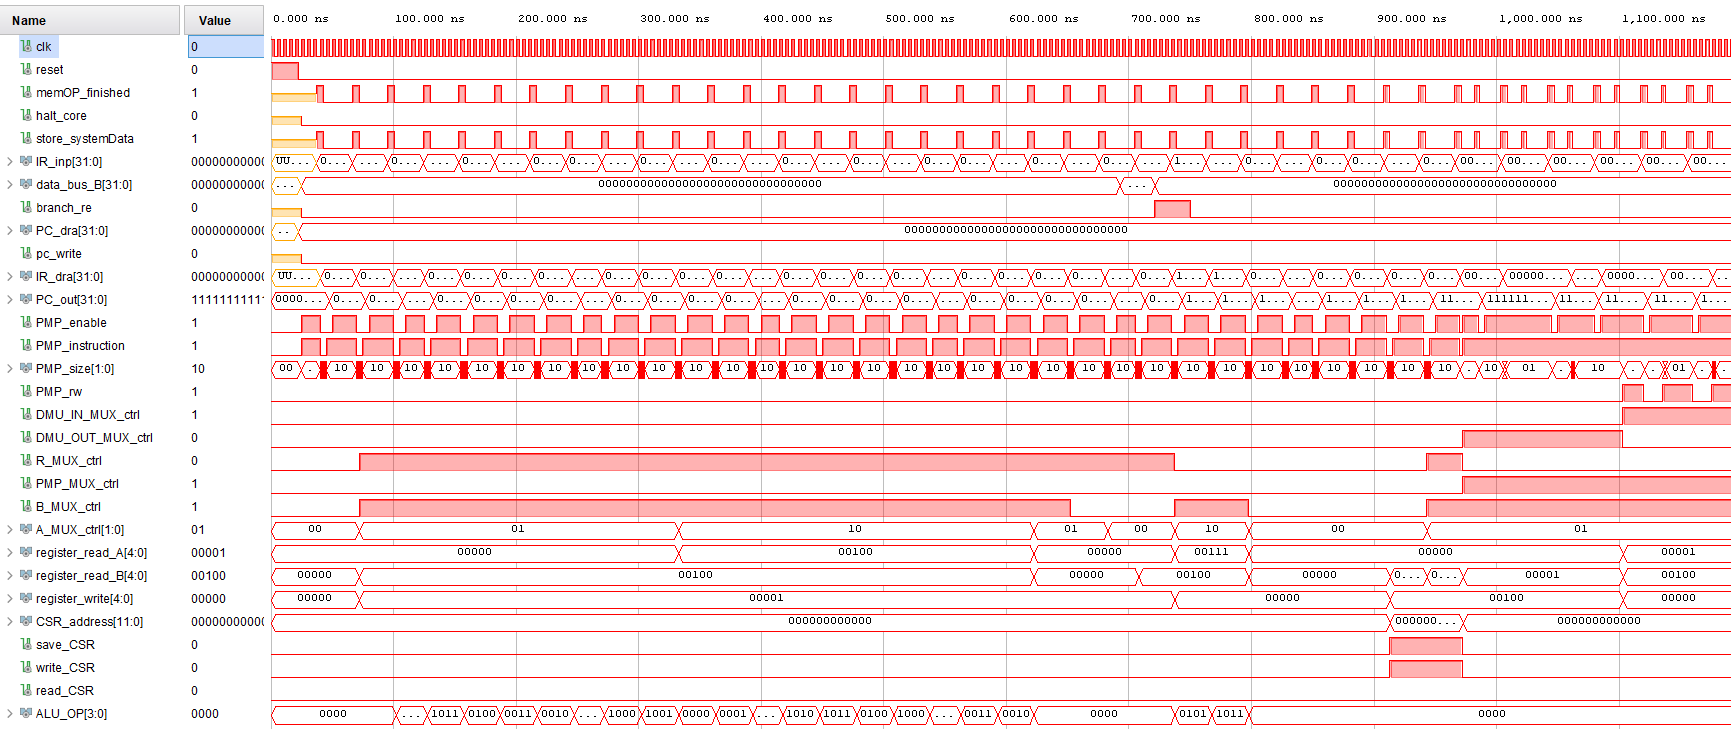
\includegraphics[width=\textwidth]{CUtoptiming}
	\caption{Vivado timing diagram for full CU integration testbench}
	\label{fig:cutoptiming}
\end{figure}
After carefully reviewing all of the output signals and the timing of the CU, the CU integration can be validated. After identifying a few bugs, the CU finally worked as it should and was ready for the next step of Test and Verification.

\section{System Verification}
After successful unit and integration verification, the entire system must be verified. This is done in Simulation to ensure that the system works before performing synthesis and \ac{PaR} to map the core in a \ac{FPGA}.\\
There are basically two ways to do this. Designated tools exist to test a custom RISC-V core for its functionality. These often require a specific debug interface such as the RISC-V External Debug Support: \cite{riscv:debug}. An example for such a verification IP is the Imperas RISC-V Reference Model. Due to the not implemented debug interface as well pressure of time to verify the functionality, another approach for system verification was chosen. \\
The basic idea is to write a simple test code and define the expected machine state after execution of said code. The code can be written in assembly and assembled using the RISC-V gcc compiler, or any other feasible compiler such as clang. A list of available compilers and software tools can be found at \cite{RV:software}. This test code is then executed in simulation.\\
In order to execute the code a test bench is implemented, containing a the \ac{EDRICO} \ac{IP}, an instruction \ac{ROM}, data \ac{RAM} and a tester \ac{RTL} module. The tester is added to the design in order to provide the proper reset and clock signals. As an additional feature it can be configured to check the machine status after execution and display status messages.\\
Debug outputs are added to the \ac{EDRICO} \ac{IP} for every register inside the \ac{RF} block as well as the \ac{IR} and \ac{PC}. The test bench also contains an AXI inteconnect, this allows to connect multiple s to a single AXI-master. The interconnect is, as well as the \ac{RAM} and \ac{ROM}, an \ac{IP} block provided by Xilinx. The test bench can be found in the appendix.\\
Figure \ref{fig:SysVerMM} shows the memory map of the test bench.


\begin{figure}[H]
	\centering
	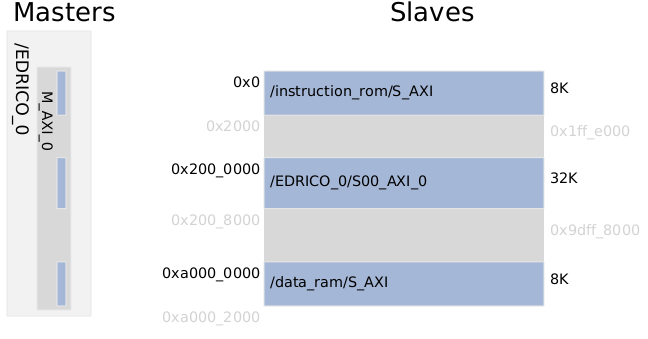
\includegraphics[width=\textwidth]{SysVer_memoryMap.png}
	\caption{memory map of the system verification test bench}
	\label{fig:SysVerMM}
\end{figure}

The instruction \ac{ROM} is defined to start at address 0x00000000 it has a size of 8KB. This is sufficient, since the test cases contain a fairly small amount of code to be executed. The same applies to the 8KB data memory at the base address of 0xA0000000.\\
In between data and instruction memory, a 32KB address space is reserved for the memory mapped \ac{CSR}.\\
\\
The test code is written in assembly, it is designed to test every RV32I instruction that is implemented. Therefore in this first test, no Zicsr instructions are tested. Hence only the \ac{GPR} and \ac{PC} contents need to be verified after execution. The \ac{IR} does not need verification, since any error in it will cause the machine to work in an undefined state, which would modify contents of the other registers to be unequal to the expected outcome.\\
Table \ref{SysVer_results} compares expected and actual register values:

\begin{table}[H]
	\setlength\arrayrulewidth{2pt}
	\centering
	\resizebox{\textwidth}{!}{
	\begin{tabular}{|c|c|c|c|c|c|}
		\rowcolor{light-gray}
		\hline
		\textbf{Register} & \textbf{Expected}  & \textbf{Actual} & \textbf{Register} & \textbf{Expected} & \textbf{Actual} \\
		\hline
		PC & 0x000000C0 & 0x00000000 & x16 & 0x0A000000 & 0x0A000000 \\
		\hline
		x1 & 0xA0000000 & 0xA0000000 & x17 & 0x00010000 & 0x00010000 \\
		\hline
		x2 & 0xC0BAD000 & 0xC0BAD000 & x18 & 0x00000000 & 0x00000000 \\
		\hline
		x3 & 0x12345000 & 0x12345000 & x19 & 0x00000001 & 0x00000001 \\
		\hline
		x4 & 0x00001000 & 0x00001000 & x20 & 0xC0BAC000 & 0xC0BAC000 \\
		\hline
		x5 & 0x000000AB & 0x000000AB & x21 & 0xC0BAD000 & 0xC0BAD000 \\
		\hline
		x6 & 0x12345014 & 0x12345014 & x22 & 0x00000000 & 0x00000000 \\
		\hline
		x7 & 0x0000C0BA & 0x0000D000 & x23 & 0x12344000 & 0x12344000 \\
		\hline
		x8 & 0x000000C0 & 0x00000000 & x24 & 0xD2EF2000 & 0xD2EF2000 \\
		\hline
		x9 & 0x12345000 & 0x13450000 & x25 & 0xF4000000 & 0xF4000000 \\
		\hline
		x10 & 0xFFFFC0BA & 0xFFFFD000 & x26 & 0x28000000 & 0x28000000 \\
		\hline
		x11 & 0xFFFFFFC0 & 0x00000000 & x27 & 0x00010000 & 0x00010000 \\
		\hline
		x12 & 0x00000000 & 0x00000000 & x28 & 0x00000000 & 0x00000000 \\
		\hline
		x13 & 0x123451EA & 0x123451EA & x29 & 0x00000001 & 0x00000001 \\
		\hline
		x14 & 0x00000004 & 0x00000004 & x30 & 0xA0000100 & 0xA0000100 \\
		\hline
		x15 & 0xFA000000 & 0xFA000000 & x31 & 0x000000B8 & 0x000000B8 \\
		\hline
	\end{tabular}}
	\label{SysVer_results}
	\caption{System Verification results and expected values}
\end{table}

The test code is made up of 48 instructions, therefore the PC is expected to be:
$$PC=48*4=192=0xC0$$
after execution. When taking a look at table \ref{SysVer_results} one sees a difference between the expected and actual result for the PC. This problem is caused by the last instruction that is executed. It is a jump back to the start of the address, hence 0x00000000. After investigating the assembly code, the cause for this behavior is found. The last instruction is a \ac{JALR} instruction.

\begin{lstlisting}[caption=Snippet 1 from the executed test code]
	JAL x31, 8 #jump 8 byte
	NOP
	JALR x0, x0, 0 #jump to start
\end{lstlisting}

Therefor the \ac{PC} is set to 0x00000000. Using the simulators waveform viewer, it can be verified that the \ac{PC} prior to this instruction was set to 0x000000BC. This confirms the correct behavior of the program counter register during execution.\\
Comparing the remaining results in the table shows another error at registers x7,x8, x10 and x11. The instructions responsible for these registers are shown below:

\begin{lstlisting}[caption=Snippet 2 from the executed test code]
	SW x2, 0(x1)
	SW x3, 4(x1)
	SW x4, 8(x1)
	ADDI x5, x0, 0xAB
	SB x5, 13(x1)
	SH x2, 14(x1)
	
	LB x11, 3(x1) #expect 0xFFFFFFC0
	LH x10, 2(x1) #expect 0xFFFFC0BA
	LW x9, 4(x1) #expect 0x12345000
	LBU x8, 3(x1) #expect 0x000000C0
	LHU x7, 2(x1) #expect 0x0000C0BA
\end{lstlisting}

This code snippet shows how the memory at base address x1 is modified by multiple store word, half-word and byte instructions.
In the second part of the code x11 to x7 are modified by load instructions. It is interesting to note, that only x9 contains the expected results, and that the instruction modifying x9 is a load word instruction. To see if the error is caused by the load instructions or if the store instructions are wrong, the memory is checked. Figure \ref{fig:SysVerWV} shows the memory in the simulation wave form view:

\begin{figure}[H]
	\centering
	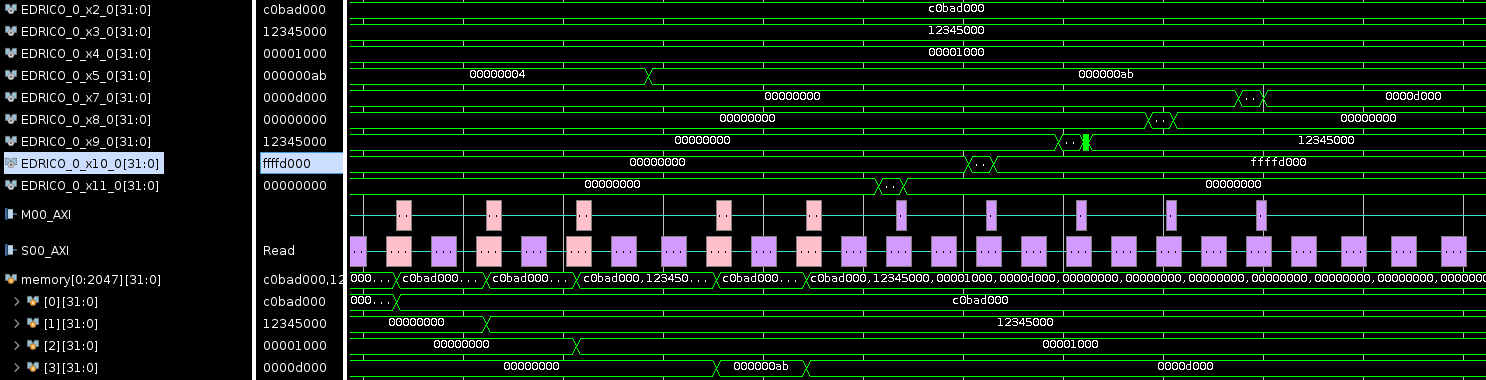
\includegraphics[width=\textwidth]{sim_EDRICO_AV_3.png}
	\caption{wave from view of the memory, AXI4-Lite transfer, x2-x5 and x7-x11 during System Verification}
	\label{fig:SysVerWV}
\end{figure}

The write transfers are displayed in the light pink-orang-ish colour whereas reads are marked in purple. As verified by comparing the memory contents with the registers x2-x4, all three store word operations are executed correctly. The store byte operation to the 0xA000000D should load 0x0000AB00 into the third memory array, followed by a store half-word to 0xA000000E which should modify the memory contents to be 0xD000AB000. However, the fourth memory element is set to 0x000000AB instead of 0x0000AB00. This is then again overwritten to be 0x0000D000. When taking a closer look at the AXI transfer everything seems fine, the right write addresses are specified and the write strobe signal (which indicates what bytes of the transfer are valid) is correct.\\
This leads to the conclusion that the mismatch in expected and actual data is not caused by the core itself. Much rather the used memory is not properly byte but word addressable. Future tests must verify this.\\
\\
One important measured value to compare processor performances is the \ac{CPI}, hence the amount of clock cycles are needed to execute an instruction. As described earlier, the \ac{CPI} is calculated using the values of the \textit{mcycle} and \textit{minstret} registers:

$$CPI = \frac{mcycleH>>32 + mcycle}{minstretH>>32 + minstret} = \frac{0x207}{0x2b} = 12.07$$

Hence in average every instruction takes 12.07 clock cycles to execute. Of course this value is highly dependent on the ratio of load/store instructions to other operations. An instruction accessing memory takes 18 cycles, whereas normal operations take 10 clock cycles. Therefore improving memory access time will decrease the CPI. Of course this assumption is very vague since, according to Amdahl's law, the improvement will not be linear \cite{patterson:2017}.
